\documentclass[10pt,letterpaper]{article}
\usepackage[top=0.85in,left=2.75in,footskip=0.75in]{geometry}
\usepackage{amsmath,amssymb}
\usepackage{nameref,hyperref}
\usepackage{array}
\usepackage{booktabs}
\usepackage{longtable}
\usepackage{graphicx}
\usepackage[aboveskip=1pt,labelfont=bf,labelsep=period,justification=raggedright,singlelinecheck=off]{caption}
\renewcommand{\figurename}{Fig}
\bibliographystyle{plos2025}
\makeatletter
\renewcommand{\@biblabel}[1]{\quad#1.}
\makeatother
\raggedright
\setlength{\parindent}{0.5cm}
\textwidth 5.25in
\textheight 8.75in
\pagestyle{plain}
\begin{document}
\vspace*{0.2in}
\begin{flushleft}
{\Large\textbf{A CPU-feasible benchmark for calibrated biomedical abstract sentence classification with external validation}}
\newline
Terry Yu\textsuperscript{1*}
\\
\bigskip
\textbf{1} [AFFILIATION TO BE COMPLETED BY AUTHOR]
\\
\bigskip
* [CORRESPONDING AUTHOR EMAIL TO BE COMPLETED BY AUTHOR]
\end{flushleft}

\section*{Abstract}
Biomedical abstract sentence classification can support evidence triage by helping researchers locate sentences that report findings or conclusions. This study evaluated whether CPU-feasible classical and recurrent neural text classifiers can identify findings/conclusion sentences in public biomedical abstracts with useful discrimination, transparent calibration assessment, and external validation. PubMed-PICO official train, validation, and test splits were used as the primary corpus, mapping R and C labels to the positive class. PubMed 20k RCT official test sentences were used only for external validation, mapping RESULTS and CONCLUSIONS to the positive class. Models included a majority baseline, TF-IDF logistic regression, TF-IDF linear support vector machine, feed-forward average embeddings, LSTM, BiLSTM, and BiLSTM with dropout. The validation-selected model was TF-IDF logistic regression. It achieved validation ROC AUC 0.977, internal test ROC AUC 0.976 (95\% bootstrap CI 0.975 to 0.977), PR AUC 0.967, F1 0.916, Brier score 0.055, and expected calibration error 0.011. External validation ROC AUC was 0.948, PR AUC 0.947, F1 0.879, Brier score 0.085, and expected calibration error 0.024. A strong sparse linear model met the empirical AUC target and performed at least as well as lightweight recurrent neural alternatives. External validation supported partial generalisation within biomedical abstracts but showed calibration degradation, so the model should be treated as a reproducible evidence-triage benchmark rather than a deployment-ready clinical system.

\section*{Keywords}
healthcare NLP; biomedical text classification; recurrent neural networks; calibration; external validation; reproducible machine learning; clinical decision support; model evaluation

\clearpage
\newgeometry{top=0.85in,left=1in,right=1in,footskip=0.75in}
\section*{Introduction}
Biomedical abstracts are a compact but information-dense substrate for evidence synthesis. In randomized-trial and clinical-research abstracts, sentences describing outcomes, findings, and conclusions are often the first targets for screening, triage, and downstream evidence extraction. A sentence-level model that can identify this rhetorical content is not a substitute for full critical appraisal, but it can reduce the cost of navigating large search results and make subsequent human review more efficient.

The methodological question is not only whether a model can obtain high discrimination. In healthcare-adjacent machine learning, calibrated probabilities and external validation are central safeguards against over-interpreting a model's apparent performance. A model that ranks sentences well may still provide misleading probability estimates, and a model tuned on one corpus may degrade when evaluated on another corpus with different labelling conventions. This study therefore treats calibration, external validation, and reproducibility as first-class outcomes.

CPU-feasible modelling is also scientifically important. Not every clinical informatics group or evidence-synthesis team has access to local GPU infrastructure, and not every biomedical NLP task requires a large Transformer model. Sparse linear models and lightweight recurrent neural networks remain attractive when a benchmark must be transparent, rerunnable, and inexpensive. This study asks whether such methods can solve a clinically meaningful abstract triage task under explicit CPU-only constraints.

The contributions are fourfold. First, the study defines a binary findings/conclusion detection task using public PubMed-PICO data and a label-compatible PubMed RCT external validation corpus. Second, it compares full-training TF-IDF baselines against CPU-limited neural models, including LSTM and BiLSTM variants. Third, it reports discrimination, thresholded classification performance, calibration metrics, reliability plots, and subgroup analysis from saved predictions. Fourth, it packages code, logs, metrics, tables, figures, and LaTeX source to support independent checking.

\section*{Related work}
Healthcare NLP has a long methodological base in converting unstructured biomedical and clinical text into analyzable evidence. General introductions and reviews emphasize both the promise of text mining and the fragility of systems that are evaluated only in narrow settings~\cite{nadkarni2011nlp,zweigenbaum2007frontiers,kreimeyer2017nlpsystems,wang2018clinicalie}. Restricted clinical-note resources and shared tasks such as MIMIC-III and i2b2/VA have shaped clinical NLP, but they require credentialed access or task-specific permissions and were therefore not used in this public CPU-only project~\cite{johnson2016mimic,uzuner2011i2b2}.

Public biomedical abstract corpora have made sentence classification a reproducible benchmark problem. PubMed-PICO was introduced for PICO element detection in medical text and has been used to study neural sentence classification with long short-term memory networks~\cite{jin2018pico}. PubMed 20k/200k RCT provides section-labelled randomized-trial abstracts for sequential sentence classification~\cite{dernoncourt2017pubmed}. EBM-NLP and related work show the broader value of patient, intervention, outcome, and evidence-bearing sentence annotations for systematic-review support~\cite{nye2018ebmnlp,kim2011ebm}. NICTA-PIBOSO is a manually annotated corpus of medical abstracts~\cite{amini2018nicta}, but it was not usable as an automatic external validation source in this run because the accessible archive did not contain usable files and the latest record was restricted. Other public biomedical tasks, including PubMedQA~\cite{jin2019pubmedqa} and adverse-event extraction corpora~\cite{gurulingappa2012ade}, were considered but were less directly aligned with a CPU-feasible calibrated binary sentence-classification benchmark.

The evidence-synthesis literature also motivates this task. Automated citation screening, review automation, and risk-of-bias systems show how NLP can reduce workload while still requiring transparent human oversight~\cite{cohen2006workload,tsafnat2014automation,marshall2014risk,marshall2015risk,marshall2015robotreviewer}. The present study is narrower than full systematic-review automation: it tests sentence-level rhetorical detection rather than eligibility, effect-size extraction, or risk-of-bias judgment.

Classical machine-learning methods remain strong baselines for text classification. TF-IDF term weighting and machine-learning text categorization have a long empirical history~\cite{salton1988term,sebastiani2002text}, and support vector machines provide a well-established margin-based classifier~\cite{cortes1995svm,joachims1998text}. Efficient linear solvers and probabilistic calibration methods make sparse models practical for large biomedical corpora~\cite{fan2008liblinear,platt1999probabilistic}. The classical models in this study were implemented with scikit-learn~\cite{pedregosa2011sklearn}.

Recurrent neural networks provide a contrasting sequence-aware modelling family. LSTM architectures were designed to address long-range dependency learning in sequential data~\cite{hochreiter1997lstm}, and bidirectional recurrent networks can incorporate context from both token directions~\cite{schuster1997brnn}. Static word vectors, convolutional sentence models, contextual embeddings, and Transformer language models have substantially shaped modern NLP~\cite{mikolov2013word2vec,kim2014cnn,peters2018elmo,vaswani2017attention,devlin2019bert}. Biomedical and scientific variants such as SciBERT, BioBERT, and PubMedBERT further demonstrate the value of domain-specific pretraining~\cite{beltagy2019scibert,lee2020biobert,gu2021pubmedbert}. This benchmark nevertheless focused on LSTM/BiLSTM neural baselines because they are realistic CPU-only comparators; GPU-scale Transformer fine-tuning was outside scope.

Evaluation in this setting must go beyond accuracy. The Brier score is a proper scoring rule for probabilistic forecasts~\cite{brier1950verification}, ROC and precision-recall analyses capture complementary aspects of binary discrimination~\cite{fawcett2006roc,davis2006prroc,saito2015pr}, and post-hoc calibration methods were developed to convert classifier scores into better probability estimates~\cite{niculescu2005probabilities,zadrozny2002classifier,guo2017calibration}. Clinical prediction literature has argued that calibration should be assessed alongside discrimination because useful ranking is not the same as reliable probabilities~\cite{vancalster2016hierarchy,vancalster2019calibration,austin2019ici}.

Transparent reporting and reproducibility are especially important when healthcare-adjacent machine learning is evaluated on proxy labels. TRIPOD and related guidance emphasize validation, complete reporting, and cautious interpretation~\cite{collins2015tripod,moons2015tripod,luo2016mlguidelines}. FAIR data principles, reproducibility recommendations, model cards, and datasheets provide complementary expectations for documenting code, data, and model limitations~\cite{wilkinson2016fair,pineau2021reproducibility,mitchell2019modelcards,gebru2021datasheets}. Clinical AI guidance, including MI-CLAIM, SPIRIT-AI, CONSORT-AI, and DECIDE-AI, reinforces that benchmark performance is not deployment evidence~\cite{norgeot2020miclaim,rivera2020spiritai,liu2020consortai,vasey2022decideai}. Broader healthcare AI commentary similarly warns that clinical impact requires validation, workflow integration, ethics review, and prospective evaluation~\cite{rajkomar2019medicine,kelly2019challenges,chen2017prediction,wiens2019roadmap,char2018ethical,nagendran2020clinicians}.

\section*{Materials and methods}
\subsection*{Data}
The primary dataset was PubMed-PICO Detection, downloaded from the public GitHub repository. The processed primary corpus contained 257,820 training sentences, 30,878 validation sentences, and 31,270 internal test sentences. Source labels R and C were mapped to the positive class, named findings/conclusion, while all other PubMed-PICO labels were mapped to the negative class. The text field was the sentence text extracted from biomedical abstracts.

External validation used the official PubMed 20k RCT test split. This corpus contributed 30,135 external sentences. Labels RESULTS and CONCLUSIONS were mapped to the positive class, and all other section labels were mapped to the negative class. This mapping is label-compatible for the narrower rhetorical construct of result or conclusion detection, not for full PICO extraction.

Official primary splits were preserved. Vectorizers, neural tokenizers, and vocabularies were fitted only on the primary training split. The validation split was used for model selection, calibration fitting, and threshold selection. The internal test split was evaluated after model selection, and the external validation split was never used for fitting, tuning, calibration, or threshold selection. Table~\ref{tab:dataset} summarises the dataset characteristics and class balance.

\begin{table}[!ht]
\centering
\caption{\textbf{Dataset characteristics.} The positive class is findings/conclusion. Text length summaries average the label-specific means and medians available in the locked evidence table.}
\begin{tabular}{llllrrr}
\hline
Dataset & Split & Total & Positive & Other & Positive \% & Median words \\
\hline
PubMed-20k-RCT & external\_test & 30135 & 14284 & 15851 & 47.4 & 23.0 \\
PubMed-PICO & test & 31270 & 13556 & 17714 & 43.4 & 21.5 \\
PubMed-PICO & train & 257820 & 111377 & 146443 & 43.2 & 21.5 \\
PubMed-PICO & validation & 30878 & 13386 & 17492 & 43.4 & 21.5 \\
\hline
\end{tabular}
\begin{flushleft}\footnotesize PubMed-PICO train, validation, and test splits were used for primary modelling. PubMed-20k-RCT external\_test was used only for external validation.\end{flushleft}
\label{tab:dataset}
\end{table}


\subsection*{Models and calibration}
The majority baseline predicted the empirical training-class prior. TF-IDF logistic regression used sparse word 1-2 grams and character 3-5 grams, with regularised logistic regression fitted on the full training split. TF-IDF linear support vector machine used the same feature family with a linear SVM and validation-fitted Platt calibration of decision scores. These baselines were included because sparse lexical models are strong, transparent, and practical under CPU-only constraints.

Neural models used a training-only vocabulary, integer token sequences, and fixed-length padded sequences. The feed-forward neural model averaged trainable token embeddings before classification. The LSTM, BiLSTM, and BiLSTM with dropout used trainable embeddings and small hidden dimensions to keep runtime feasible on CPU. Neural models were trained on a stratified cap of 120,000 training sentences, evaluated on the full validation, test, and external splits, and used early stopping based on validation performance. This cap is a methodological constraint rather than an optimization claim.

Classical models were calibrated with Platt sigmoid calibration fitted on validation scores. Neural models were calibrated with temperature scaling fitted on validation logits. Thresholds were optimized for validation F1 only. No preprocessing, calibration, threshold selection, or model selection used the internal test or external validation labels.

Experiments were conducted in CPU-only mode on Windows 11 with Python 3.14 and CPU PyTorch. CUDA availability was explicitly checked and was false. Random seeds and training logs were saved with the run artifacts.

\subsection*{Evaluation}
The primary metric was receiver operating characteristic area under the curve. Secondary metrics were precision-recall area under the curve, accuracy, sensitivity/recall, specificity, precision/positive predictive value, F1 score, confusion matrix counts, Brier score, expected calibration error, calibration intercept, and calibration slope. Reliability plots, ROC curves, precision-recall curves, and confusion matrices were generated from saved predictions.

Calibration was assessed after validation-fitted calibration. The evidence lock does not contain pre-calibration Brier scores or expected calibration errors for all models; therefore, this manuscript does not claim that calibration improved these metrics. Instead, it reports the calibrated probability performance available from the completed experiments.

External validation was performed by applying the selected training-fitted preprocessing and trained models to the PubMed 20k RCT external test split. The external data were never used for training, tuning, or threshold selection. Subgroup analysis used ethically neutral metadata available in the corpora: sentence-length quartiles. No demographic or patient-level fairness analysis was possible because the datasets do not contain such metadata.

\section*{Results}
The empirical AUC target was achieved. Table~\ref{tab:model-comparison} shows the model comparison. TF-IDF logistic regression was selected by validation ROC AUC, with validation ROC AUC 0.977, Brier score 0.054, and expected calibration error 0.012. On the internal test split, the same model achieved ROC AUC 0.976 (95\% bootstrap CI 0.975 to 0.977), PR AUC 0.967, accuracy 0.926, F1 0.916, sensitivity 0.935, specificity 0.918, Brier score 0.055, and expected calibration error 0.011. The internal-test confusion matrix for the selected threshold contained 12,681 true positives, 16,266 true negatives, 1,448 false positives, and 875 false negatives.

\begin{table}[!ht]
\centering
\caption{\textbf{Model comparison on validation and internal test splits.} Model selection used validation ROC AUC, with Brier score as a secondary calibration criterion.}
\small
\begin{tabular}{lrrrrrr}
\hline
Model & Val AUC & Test AUC & Test PR AUC & Test F1 & Test Brier & Test ECE \\
\hline
bilstm & 0.975 & 0.974 & 0.965 & 0.908 & 0.060 & 0.010 \\
bilstm\_dropout & 0.965 & 0.964 & 0.953 & 0.893 & 0.071 & 0.015 \\
ffnn\_avg\_embeddings & 0.962 & 0.962 & 0.948 & 0.887 & 0.074 & 0.010 \\
lstm & 0.892 & 0.891 & 0.886 & 0.800 & 0.129 & 0.039 \\
majority\_baseline & 0.500 & 0.500 & 0.434 & 0.000 & 0.246 & 0.002 \\
tfidf\_linear\_svm & 0.976 & 0.974 & 0.964 & 0.915 & 0.057 & 0.011 \\
tfidf\_logistic\_regression & 0.977 & 0.976 & 0.967 & 0.916 & 0.055 & 0.011 \\
\hline
\end{tabular}
\begin{flushleft}\footnotesize All values are from saved run metrics. Classical models used validation-fitted Platt calibration; neural models used validation-fitted temperature scaling.\end{flushleft}
\label{tab:model-comparison}
\end{table}


The strongest neural model was the BiLSTM, with internal test ROC AUC 0.974, compared with 0.976 for TF-IDF logistic regression and 0.974 for TF-IDF linear SVM. The unidirectional LSTM was weaker, with internal test ROC AUC 0.891. This pattern indicates that lightweight recurrence did not provide a clear advantage over sparse lexical baselines under the CPU-feasible protocol.

Table~\ref{tab:calibration} reports calibrated probability metrics. The selected model's internal calibration was strong by the saved metrics, with internal-test Brier score 0.055, expected calibration error 0.011, calibration intercept -0.021, and calibration slope 0.983. External calibration was weaker, with Brier score 0.085, expected calibration error 0.024, and calibration slope 0.770, consistent with corpus and label shift.

\begin{table}[!ht]
\centering
\caption{\textbf{Post-calibration probability metrics.} Pre-calibration Brier and ECE were not saved for all models and are therefore not reported.}
\small
\begin{tabular}{llrrrr}
\hline
Model & Split & Post Brier & Post ECE & Calibration intercept & Calibration slope \\
\hline
bilstm & validation & 0.059 & 0.010 & -0.171 & 1.006 \\
bilstm & test & 0.060 & 0.010 & -0.161 & 0.997 \\
bilstm & external & 0.100 & 0.042 & 0.075 & 0.737 \\
bilstm\_dropout & validation & 0.070 & 0.016 & 0.174 & 1.011 \\
bilstm\_dropout & test & 0.071 & 0.015 & 0.189 & 1.008 \\
bilstm\_dropout & external & 0.120 & 0.060 & 0.414 & 0.756 \\
ffnn\_avg\_embeddings & validation & 0.074 & 0.011 & -0.152 & 1.002 \\
ffnn\_avg\_embeddings & test & 0.074 & 0.010 & -0.128 & 1.003 \\
ffnn\_avg\_embeddings & external & 0.119 & 0.037 & 0.239 & 0.784 \\
lstm & validation & 0.128 & 0.039 & 0.447 & 1.156 \\
lstm & test & 0.129 & 0.039 & 0.435 & 1.148 \\
lstm & external & 0.169 & 0.097 & 0.656 & 0.981 \\
majority\_baseline & validation & 0.246 & 0.002 & -0.249 & 0.068 \\
majority\_baseline & test & 0.246 & 0.002 & -0.249 & 0.068 \\
majority\_baseline & external & 0.251 & 0.042 & -0.097 & 0.027 \\
tfidf\_linear\_svm & validation & 0.055 & 0.011 & 0.000 & 1.001 \\
tfidf\_linear\_svm & test & 0.057 & 0.011 & -0.009 & 0.985 \\
tfidf\_linear\_svm & external & 0.088 & 0.025 & 0.024 & 0.763 \\
tfidf\_logistic\_regression & validation & 0.054 & 0.012 & -0.000 & 1.000 \\
tfidf\_logistic\_regression & test & 0.055 & 0.011 & -0.021 & 0.983 \\
tfidf\_logistic\_regression & external & 0.085 & 0.024 & 0.007 & 0.770 \\
\hline
\end{tabular}
\begin{flushleft}\footnotesize Calibration method: Platt sigmoid calibration for TF-IDF logistic regression and linear SVM; temperature scaling for neural models; none for the majority baseline. The evidence lock does not support any claim that calibration improved Brier score or ECE because pre-calibration metrics were not retained.\end{flushleft}
\label{tab:calibration}
\end{table}


External validation results are shown in Table~\ref{tab:external}. The selected model achieved external ROC AUC 0.948, PR AUC 0.947, accuracy 0.883, and F1 0.879. The external ROC AUC was lower than internal test ROC AUC by -0.028. Table~\ref{tab:subgroup} summarises sentence-length subgroup results. Longer sentences had higher observed AUC in both internal and external splits, but these results are descriptive and should not be interpreted as clinical subgroup performance.

\begin{table}[!ht]
\centering
\caption{\textbf{External validation results.} Performance drop is external ROC AUC minus internal test ROC AUC; negative values indicate lower external discrimination.}
\small
\begin{tabular}{lrrrrrr}
\hline
Model & Test AUC & External AUC & AUC drop & External F1 & External Brier & External ECE \\
\hline
bilstm & 0.974 & 0.937 & -0.037 & 0.857 & 0.100 & 0.042 \\
bilstm\_dropout & 0.964 & 0.916 & -0.048 & 0.827 & 0.120 & 0.060 \\
ffnn\_avg\_embeddings & 0.962 & 0.912 & -0.050 & 0.828 & 0.119 & 0.037 \\
lstm & 0.891 & 0.835 & -0.057 & 0.749 & 0.169 & 0.097 \\
majority\_baseline & 0.500 & 0.500 & 0.000 & 0.000 & 0.251 & 0.042 \\
tfidf\_linear\_svm & 0.974 & 0.945 & -0.029 & 0.877 & 0.088 & 0.025 \\
tfidf\_logistic\_regression & 0.976 & 0.948 & -0.028 & 0.879 & 0.085 & 0.024 \\
\hline
\end{tabular}
\begin{flushleft}\footnotesize The external split was not used for training, hyperparameter selection, thresholding, or calibration fitting.\end{flushleft}
\label{tab:external}
\end{table}


\begin{table}[!ht]
\centering
\caption{\textbf{Sentence-length subgroup analysis for the selected model.} Subgroups are descriptive and based on length quartiles.}
\begin{tabular}{llrrrr}
\hline
Split & Group & n & ROC AUC & Brier & ECE \\
\hline
test & short & 8600 & 0.974 & 0.053 & 0.016 \\
test & medium\_short & 7404 & 0.965 & 0.069 & 0.015 \\
test & medium\_long & 7480 & 0.974 & 0.058 & 0.012 \\
test & long & 7786 & 0.984 & 0.042 & 0.014 \\
external & short & 8216 & 0.921 & 0.108 & 0.040 \\
external & medium\_short & 7154 & 0.938 & 0.095 & 0.028 \\
external & medium\_long & 7676 & 0.954 & 0.078 & 0.020 \\
external & long & 7089 & 0.970 & 0.058 & 0.018 \\
\hline
\end{tabular}
\begin{flushleft}\footnotesize All subgroup cells had large sample sizes in this run. Results should still be interpreted descriptively because length groups were not pre-specified clinical subgroups.\end{flushleft}
\label{tab:subgroup}
\end{table}


Error analysis found that false positives often involved method or outcome-definition sentences with result-like clinical endpoint language. False negatives often involved short or numerically dense findings sentences. High-confidence errors illustrated the limitation of section-heading-derived labels: some sentences can be semantically compatible with more than one rhetorical role even when the dataset assigns a single label.

\begin{figure}[!ht]
\centering
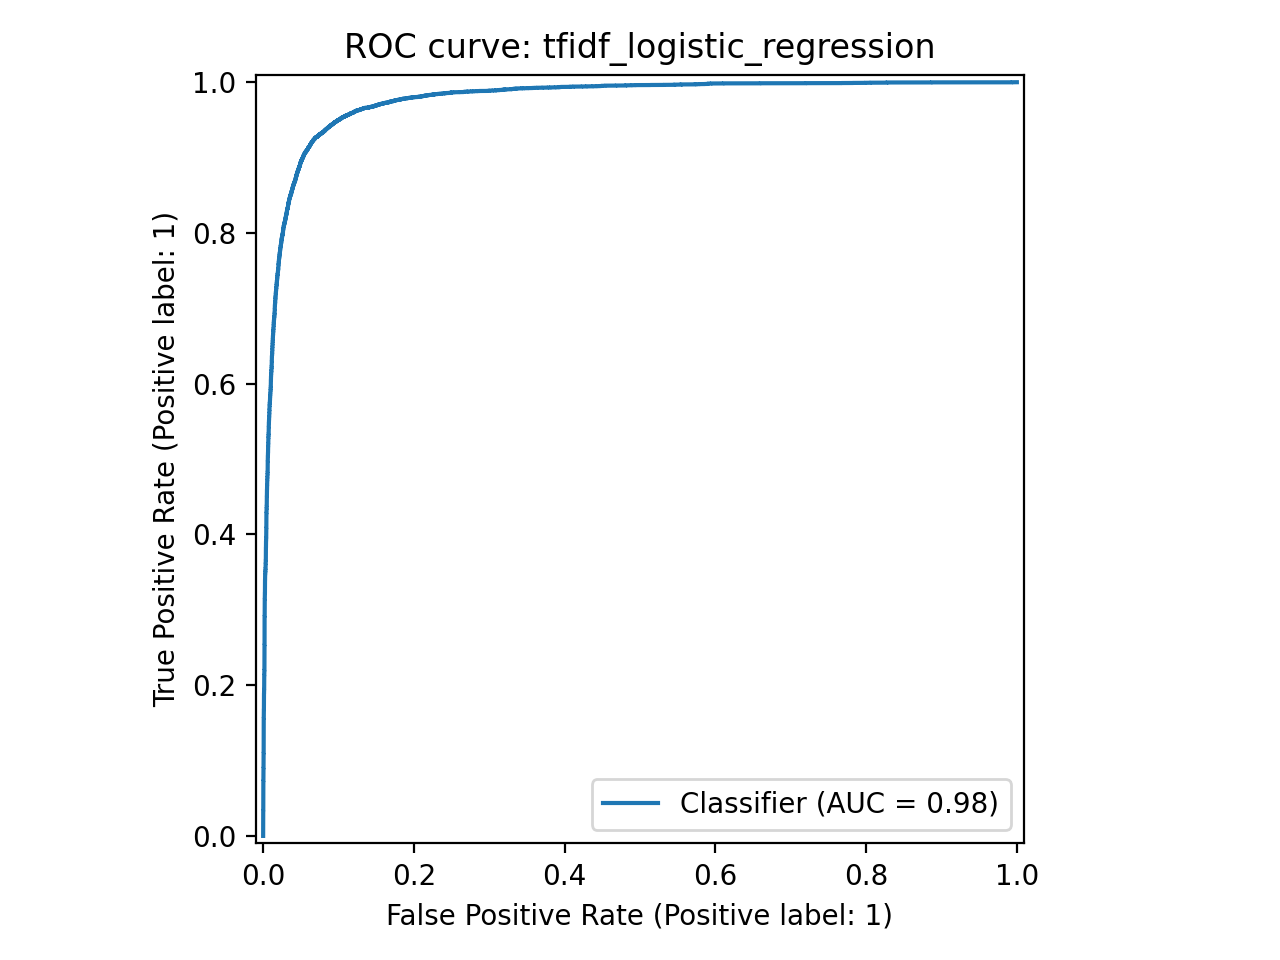
\includegraphics[width=0.72\linewidth]{figures/roc_curve_best_model.png}
\caption{\textbf{Internal test ROC curve for the validation-selected model.} The selected model was TF-IDF logistic regression.}
\label{fig:roc}
\end{figure}

\begin{figure}[!ht]
\centering
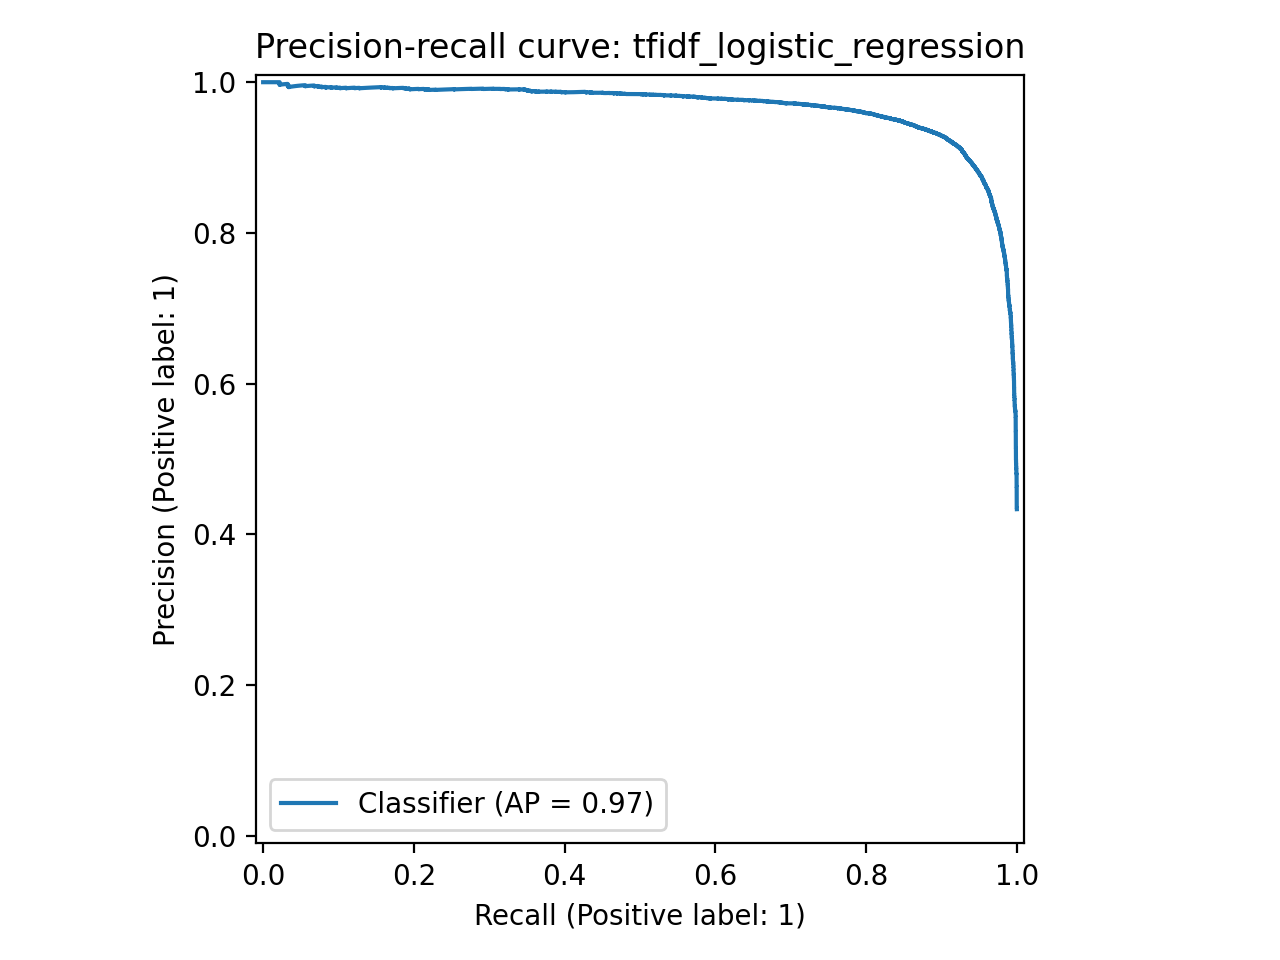
\includegraphics[width=0.72\linewidth]{figures/pr_curve_best_model.png}
\caption{\textbf{Internal test precision-recall curve for the validation-selected model.}}
\label{fig:pr}
\end{figure}

\begin{figure}[!ht]
\centering
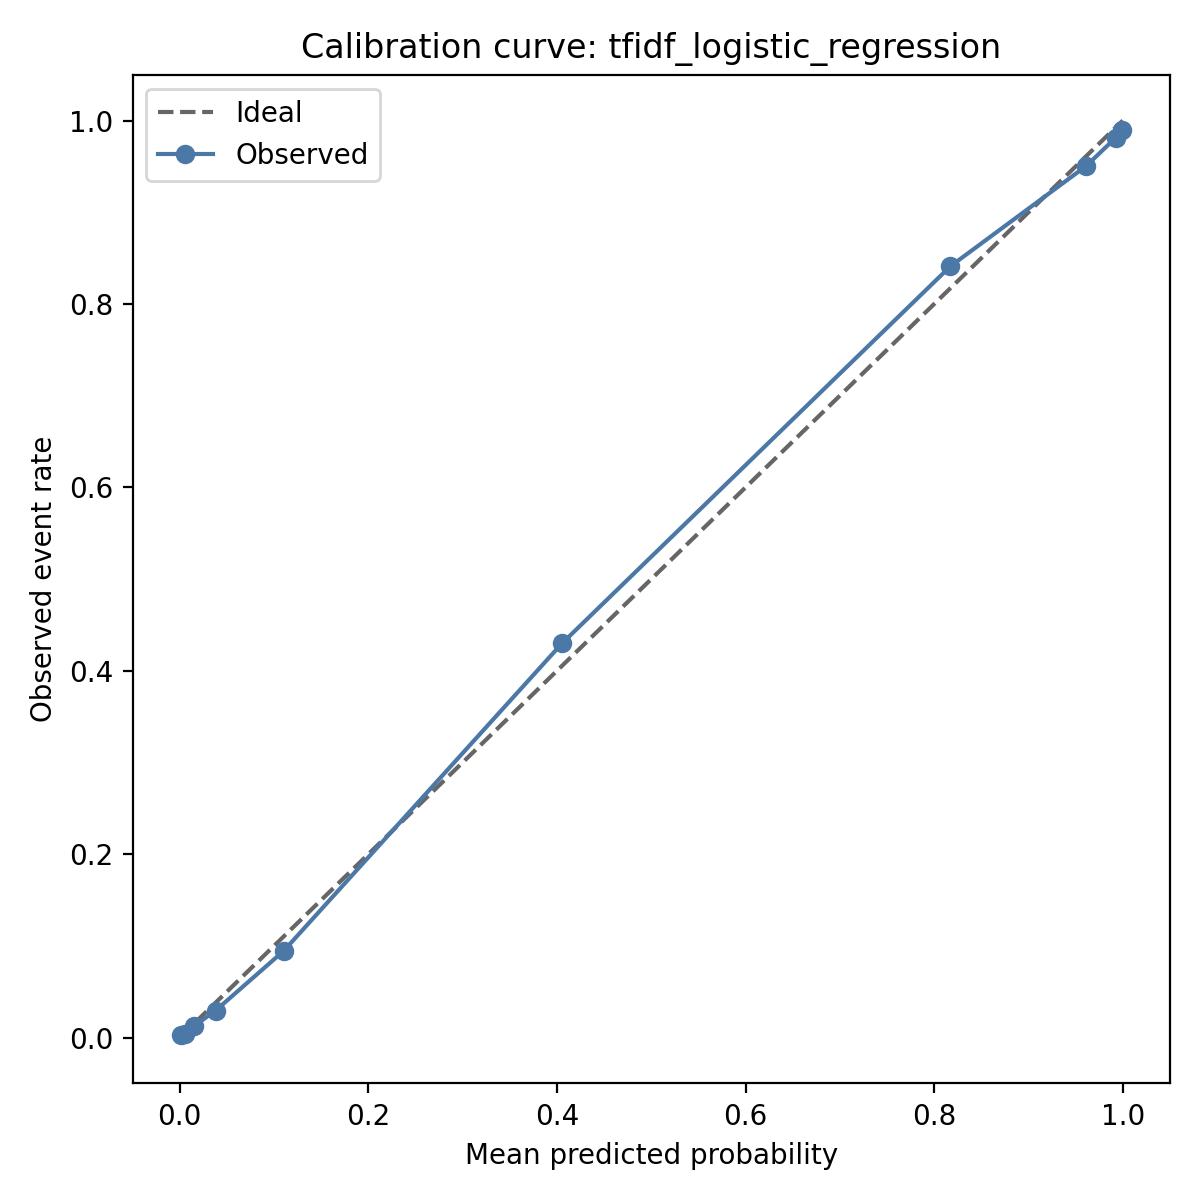
\includegraphics[width=0.72\linewidth]{figures/calibration_curve_best_model.png}
\caption{\textbf{Internal test calibration curve for the validation-selected model.}}
\label{fig:calibration}
\end{figure}

\begin{figure}[!ht]
\centering
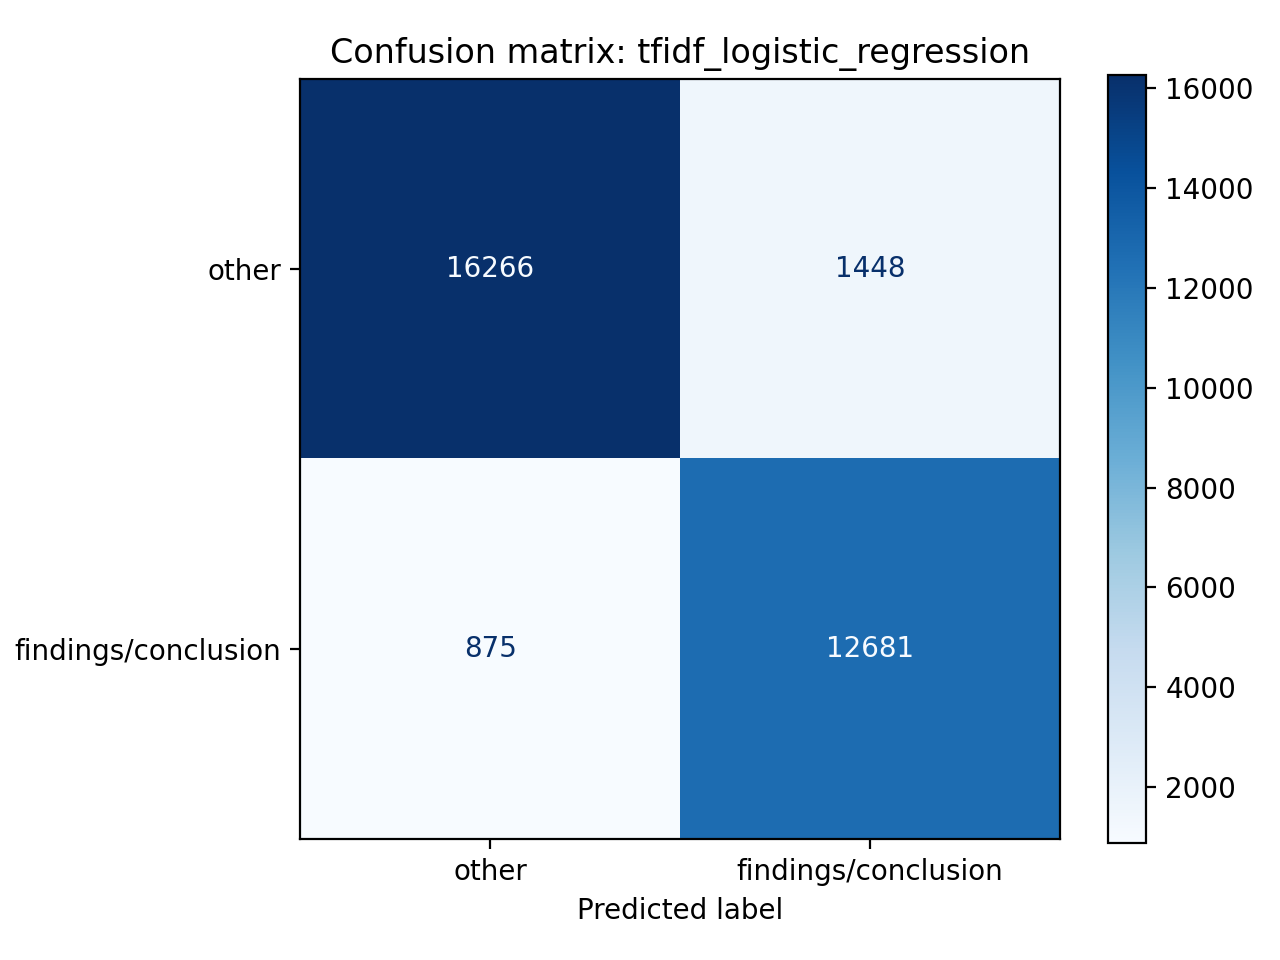
\includegraphics[width=0.72\linewidth]{figures/confusion_matrix_best_model.png}
\caption{\textbf{Internal test confusion matrix for the validation-selected model.}}
\label{fig:confusion}
\end{figure}

\begin{figure}[!ht]
\centering
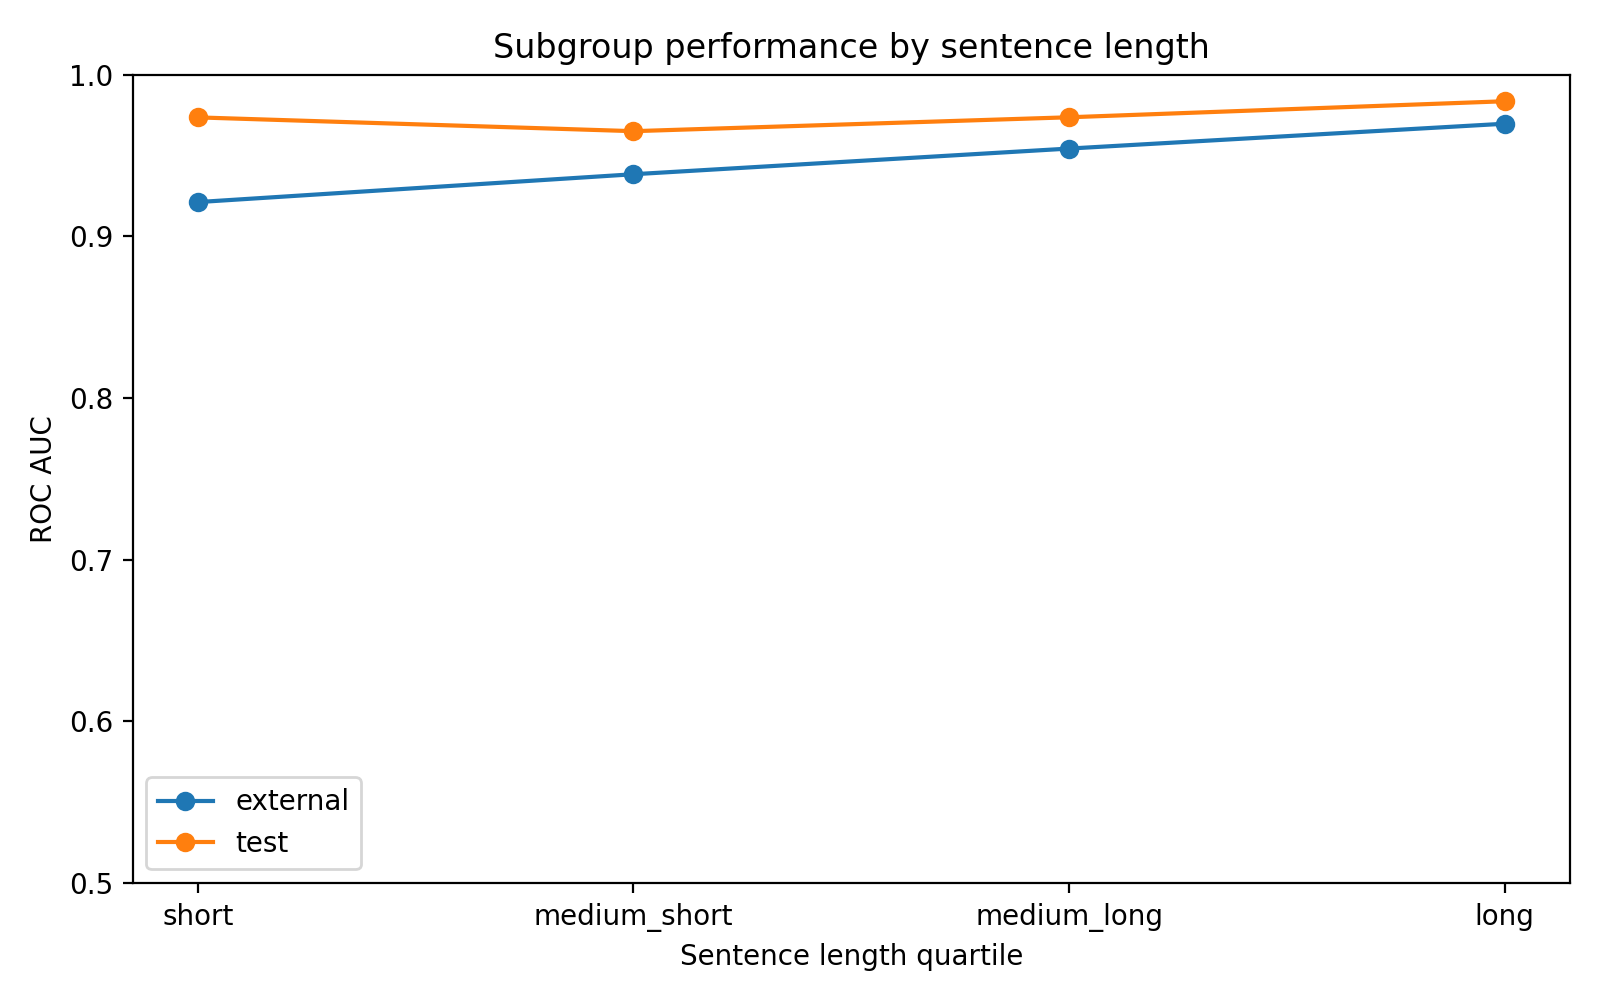
\includegraphics[width=0.72\linewidth]{figures/subgroup_performance.png}
\caption{\textbf{Sentence-length subgroup performance.} Subgroups are descriptive length quartiles.}
\label{fig:subgroup}
\end{figure}

\section*{Discussion}
This study demonstrates that a CPU-only biomedical sentence-classification benchmark can achieve strong discrimination and report useful calibration diagnostics without GPU-scale modelling. The best model was TF-IDF logistic regression rather than a recurrent neural network. This does not imply that neural models are generally inferior; rather, it shows that for this public abstract-level task, sparse lexical features capture much of the signal and provide a strong baseline that should not be skipped.

The external validation result supports partial generalisation to a related biomedical abstract corpus, but it also reveals the expected fragility of probabilities under corpus shift. Discrimination remained high externally, yet Brier score, expected calibration error, and calibration slope degraded. For evidence-triage use, this means that ranked sentence retrieval may transfer better than absolute probability interpretation. Any downstream use should consider recalibration in the target corpus and further validation with manually adjudicated labels.

The benchmark also illustrates a practical reproducibility point. CPU-feasible pipelines are easier to rerun, inspect, and package. The project saved raw and processed manifests, training logs, predictions, calibration artifacts, metrics, figures, tables, and manuscript source. This level of evidence traceability is valuable even when the model itself is methodologically simple.

Clinically, the model should not be interpreted as a decision-support system. It detects rhetorical sentence roles in abstracts. It does not assess trial quality, extract effect sizes, evaluate bias, or recommend patient care. The appropriate interpretation is a reproducible benchmark for literature triage and methodological evaluation.

\section*{Limitations}
The primary limitation is the label source. PubMed-PICO and PubMed RCT labels are derived from abstract structure or annotation conventions, and a section label is not always equivalent to sentence-level semantics. Some errors identified in the analysis likely reflect ambiguous or proxy labels rather than purely model failures.

The external validation corpus is public and held out, but it remains in the biomedical abstract domain. It is not a manually adjudicated external clinical setting, and it does not prove deployment readiness. The NICTA-PIBOSO corpus was investigated as a manual external validation candidate but was not automatically available in usable form in this environment.

The neural experiments were intentionally CPU-limited. Models used small embeddings, short maximum sequence lengths, and a stratified cap on neural training examples. Larger recurrent models, pretrained biomedical Transformers, or GPU-scale fine-tuning might perform differently, but they were outside the CPU-only scope of this project.

Calibration uncertainty is another limitation. The project reports calibrated Brier score, expected calibration error, and reliability curves, but it did not retain pre-calibration Brier/ECE for all models and did not compute uncertainty intervals for calibration metrics. No demographic fairness analysis was possible because the public abstract corpora do not include patient-level demographic metadata.

\section*{Conclusion}
A complete CPU-only healthcare NLP benchmark achieved the empirical AUC target for findings/conclusion sentence detection in biomedical abstracts, with the validation-selected TF-IDF logistic regression model obtaining internal test ROC AUC 0.976 and external ROC AUC 0.948. Lightweight recurrent neural models were feasible and informative but did not outperform the strongest sparse baseline. The results support careful, reproducible, calibration-aware benchmarking for healthcare NLP while underscoring that abstract sentence classification is not clinical deployment evidence.

\section*{Data availability statement}
The raw public datasets used in this study are available from the PubMed-PICO Detection repository (https://github.com/jind11/PubMed-PICO-Detection) and the PubMed RCT repository (https://github.com/Franck-Dernoncourt/pubmed-rct). The processed data, predictions, summary tables, and figures were generated by the local scripts in this project. Before journal submission, the author should deposit the generated minimal replication package in a public repository and replace this placeholder with a persistent URL or DOI: [REPOSITORY URL TO BE INSERTED].

\section*{Code availability statement}
The code used to download data, prepare datasets, train models, calibrate predictions, evaluate metrics, generate figures, and build the manuscript package is located in the local project directories \texttt{src/} and \texttt{scripts/}. Before submission, the author should publish the code in a public repository or archival service and insert the persistent repository URL here: [REPOSITORY URL TO BE INSERTED].

\section*{Ethics statement}
This study used public biomedical abstract datasets and did not recruit participants, contact patients, process restricted clinical notes, or deploy a model in patient care. No identifiable patient-level data were used. The models are for research evaluation and evidence-triage benchmarking only and should not be used for clinical decision-making without separate validation, governance review, and prospective evaluation.

\section*{Funding statement}
The author received no specific funding for this work. Author confirmation is needed before submission.

\section*{Competing interests}
The author declares no competing interests. Author confirmation is needed before submission.

\section*{Author contributions}
Author-confirmation-needed CRediT statement: Conceptualisation, methodology, software, formal analysis, investigation, data curation, validation, visualisation, writing--original draft, and writing--review and editing: Terry Yu.

\section*{Acknowledgements}
Not applicable.


\section*{Supporting information}
S1 Text. Supplementary methods. See \texttt{supplementary/supplementary\_methods.tex}.

S2 Text. Supplementary results. See \texttt{supplementary/supplementary\_results.tex}.

S3 Checklist. Reproducibility checklist. See \texttt{supplementary/reproducibility\_checklist.tex}.

\bibliography{references}
\end{document}
